\documentclass[12pt]{kjleehw}

\usepackage{subfigure}
\usepackage{CJKutf8}
\usepackage{listings}
\usepackage{verbatim}
\usepackage{enumerate}
\usepackage{amsmath, amsfonts, amssymb, mathtools}
\usepackage{bm}
\usepackage{pagecolor}
\usepackage{changepage}
\usepackage{listings}
% \lstset{
%   backgroundcolor=\color{gray},
% }
\definecolor{codegreen}{rgb}{0,0.6,0}
\definecolor{codegray}{rgb}{0.5,0.5,0.5}
\definecolor{codepurple}{rgb}{0.58,0,0.82}
\definecolor{backcolour}{rgb}{0.95,0.95,0.92}
\lstdefinestyle{mystyle}{
    backgroundcolor=\color{backcolour},   
    commentstyle=\color{codegreen},
    keywordstyle=\color{magenta},
    numberstyle=\tiny\color{codegray},
    stringstyle=\color{codepurple},
    basicstyle=\footnotesize,
    breakatwhitespace=false,         
    breaklines=true,                 
    captionpos=b,                    
    keepspaces=true,                 
    numbers=left,                    
    numbersep=5pt,                  
    showspaces=false,                
    showstringspaces=false,
    showtabs=false,                  
    tabsize=2
}
 
\lstset{style=mystyle}

\renewcommand{\figurename}{Figure}
\renewcommand{\tablename}{Table}

\renewcommand\appendix{\par
\setcounter{section}{0}
\setcounter{subsection}{0}\today\today
\setcounter{figure}{0}
\setcounter{table}{0}
\renewcommand\thesection{Appendix \Alph{section}}
\renewcommand\thefigure{\Alph{section}\arabic{figure}}
\renewcommand\thetable{\Alph{section}\arabic{table}}
}

\usepackage{etoolbox}
\patchcmd{\thebibliography}{\section*{\refname}}{}{}{}
% --

\setlength{\abovecaptionskip}{10pt}
\setlength{\belowcaptionskip}{10pt}

\setlength{\parindent}{0em}

% English Font and color, rm/ss/tt
\renewcommand{\familydefault}{\rmdefault} 
% \definecolor{EyeBlack}{HTML}{222222}
% \definecolor{EyeGreen}{HTML}{76D38F}
% \pagecolor{EyeBlack}
% \color{EyeGreen}

% ----
% ----

\begin{document}
\begin{CJK}{UTF8}{bkai} 
\title{\textbf{Optimization in Engineering \\ Appendix - Run ANSYS Workbench in batch mode}}
% \lhead{Optimal Design}
% \rhead{System Optimization Lab.}

% \tableofcontents

% -----------------------------------------------
\section{Introduction}

This document and example file are only used for academic purpose and released in MIT License. We demonstrate how to use batch mode with Python script to change the ANSYS Workbench's parameters (or variables), then execute the simulation and export results to a text file.

% -----------------------------------------------
\section{Install ANSYS Student}

We are \underline{\textbf{not}} encourage students to use commercial softwares without license. The ANSYS Student Software provide a twelve-month renewable license which is limited with 32k nodes/elements in Structure Analysis, 512k nodes/cells in Fluid Analysis. You can 
download it from the website : \textbf{https://www.ansys.com/academic/free-student-products}

\begin{figure}[h]
	\centering
	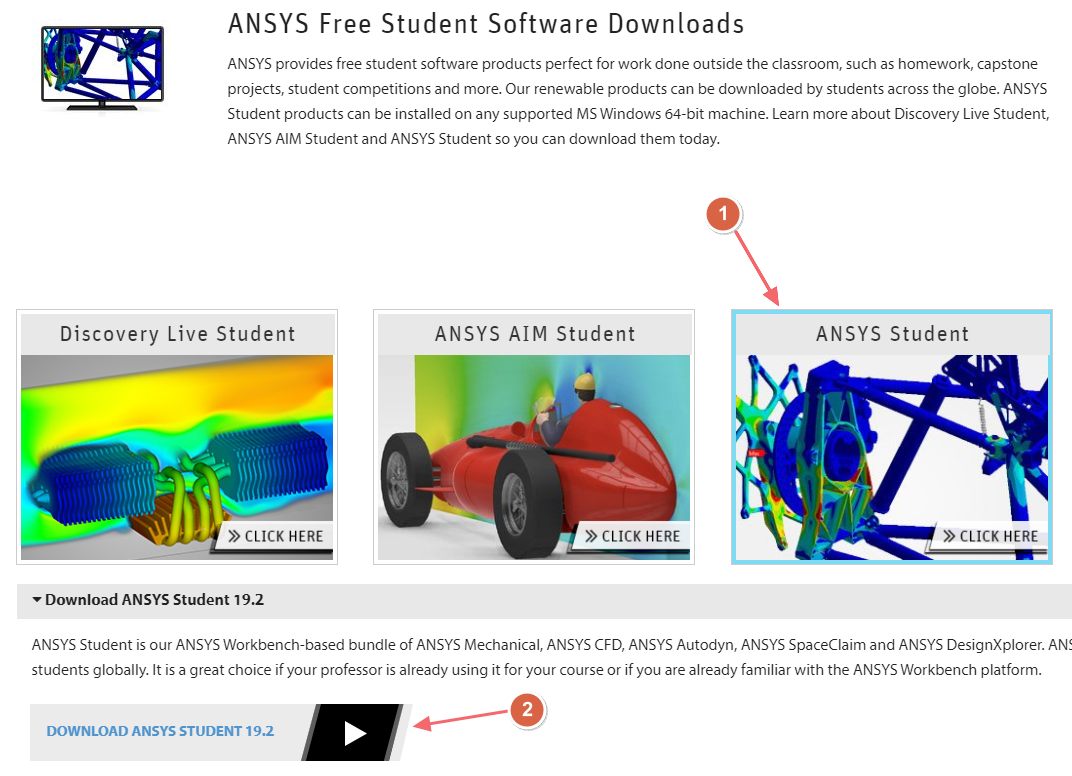
\includegraphics[scale=0.4]{figure/download_ansys.png}
	\caption{ANSYS Free Student Software Downloads}
	\label{fig:download_ansys}
\end{figure}

% -----------------------------------------------
\section{Example}

\subsection{Files}

The \textbf{example.zip} should contain at least four items which include following files/folder:

\begin{itemize}
  \item model\_v192\_student.wbpj
  \item model\_v192\_student\_files/
  \item batch\_run\_ansys.py
  \item batch\_cmd.bat
\end{itemize}

The project file (model\_v192\_student.wbpj) should only be opened in ANSYS Student v19.2 or newer version.

\subsection{Problem Description}

In this model, we construct a cantilever beam which has three sections as shown in Figure \ref{fig:cantilever}. Each section has a circle sketch and uses the diameter as the design variables.\\

\begin{figure}[h]
	\centering
	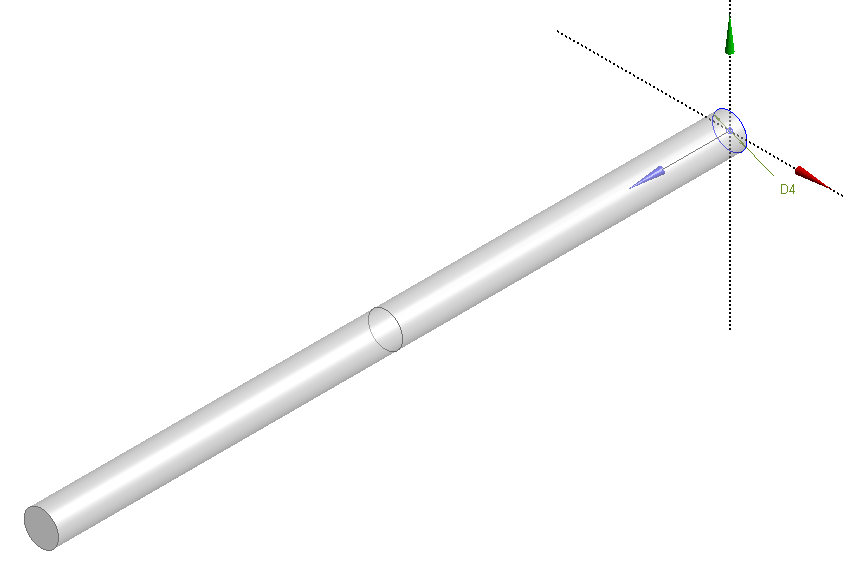
\includegraphics[scale=0.4]{figure/cantilever.png}
	\caption{Geometry}
	\label{fig:cantilever}
\end{figure}

In structural simulation, we fixed one end of the beam and apply a 100 [N] force (+x) on the other side. The stress and deformation distribution are shown in Figure \ref{fig:anslysis}. Then we can retrieve the response values to Parameter Set Table, as shown in Figure \ref{fig:parameters}.

\newpage

\begin{figure}[h]
	\centering
  \subfigure[Stress Distribution]{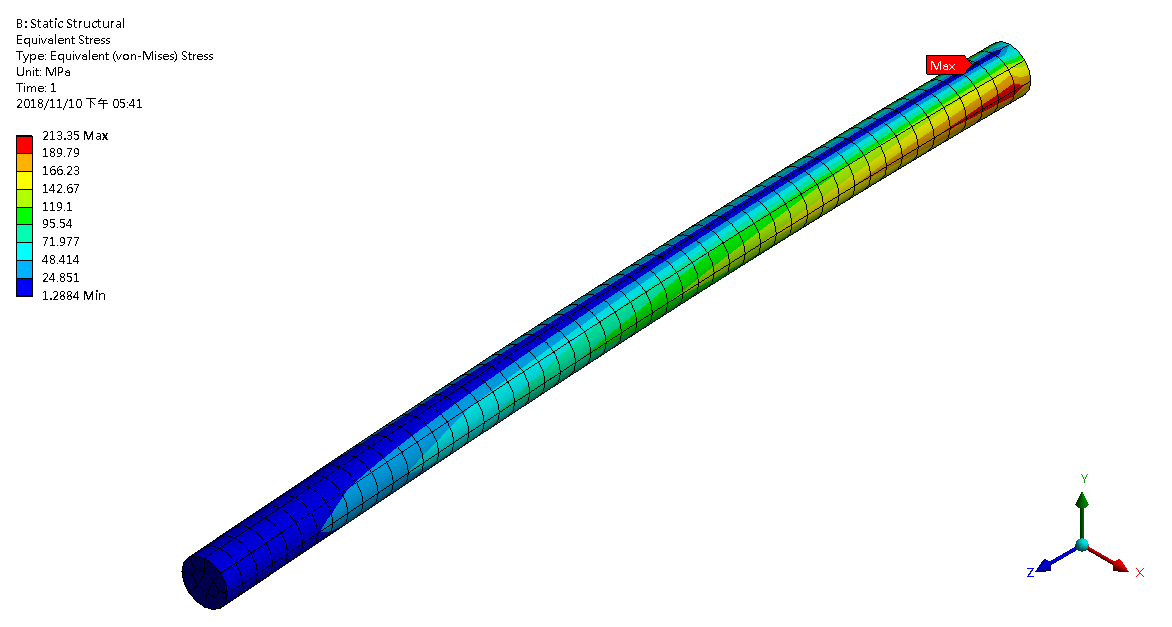
\includegraphics[height=4.2cm]{./figure/stress.png}}
  \subfigure[Max. Displacement]{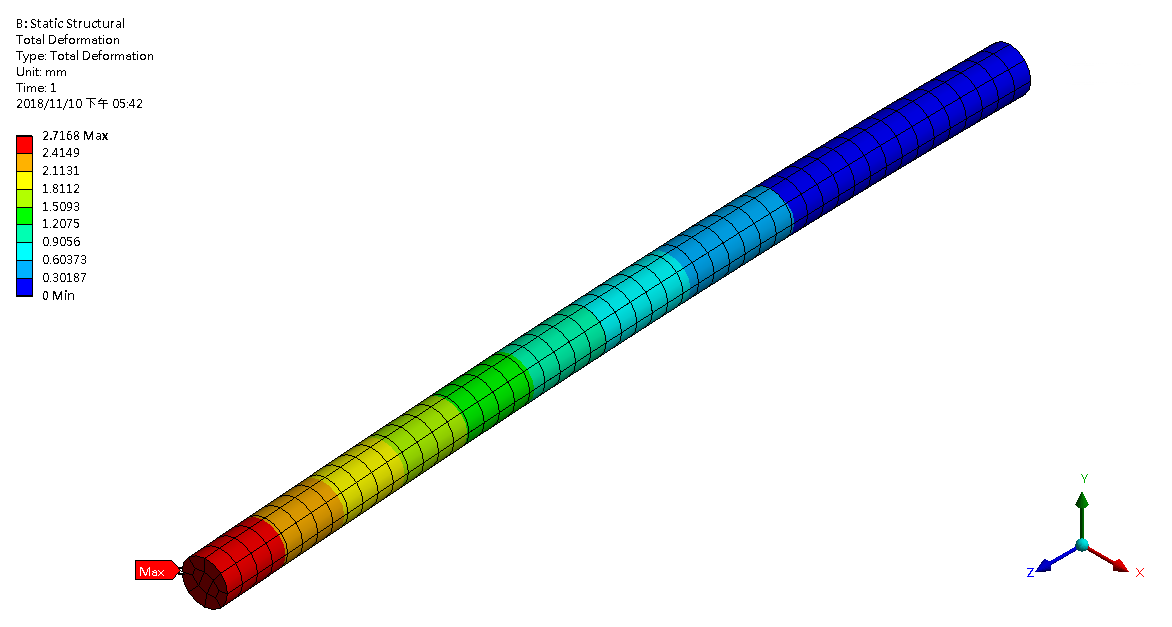
\includegraphics[height=4.2cm]{./figure/disp.png}}
  \caption{Analysis Result}
  \label{fig:anslysis}
\end{figure}

\begin{figure}[h]
	\centering
	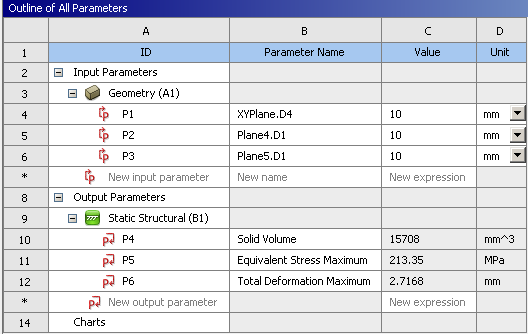
\includegraphics[scale=0.65]{figure/parameters.png}
	\caption{Parameters}
	\label{fig:parameters}
\end{figure}

\subsection{Batch Mode}

\begin{itemize}
  \item batch\_run\_ansys.py

\lstinputlisting[language=Python, firstline=1, lastline=4]{./code/batch_run_ansys.py}

You need to modify the project file's location in code line 3 before running the batch mode. This file path might be different in your computer.\\

\lstinputlisting[language=Python, firstline=5, lastline=17, firstnumber=5]{./code/batch_run_ansys.py}

Then you can decide which parameter should be changed and modify the value by the "Expression" argument.\\

\lstinputlisting[language=Python, firstline=22, lastline=30, firstnumber=22]{./code/batch_run_ansys.py}

After updating the project. Use Python file I/O function to write out the parameter's information to a text file.

\end{itemize}

\begin{itemize}
  \item batch\_cmd.bat
  \lstinputlisting[language=Python]{./code/batch_cmd.bat}

  The first part of this .bat file is the path of ANSYS WB program, and the arguement means running the program with batch\_run\_ansys.py in batch mode. This two files (batch\_run\_ansys.py and batch\_cmd.bat) should be placed in the same folder.
\end{itemize}

After executing the batch\_cmd.bat. It will appear two MS-DOS windows as shown in Figure \ref{fig:batch}, and create output.txt when it finished. The output.txt will contain the parameter's information of the project file. \\

For the detailed operation procedure, please check the video : \\
\textbf{https://www.youtube.com/watch?v=jGWYmR0uqtU}

\begin{figure}[h]
	\centering
	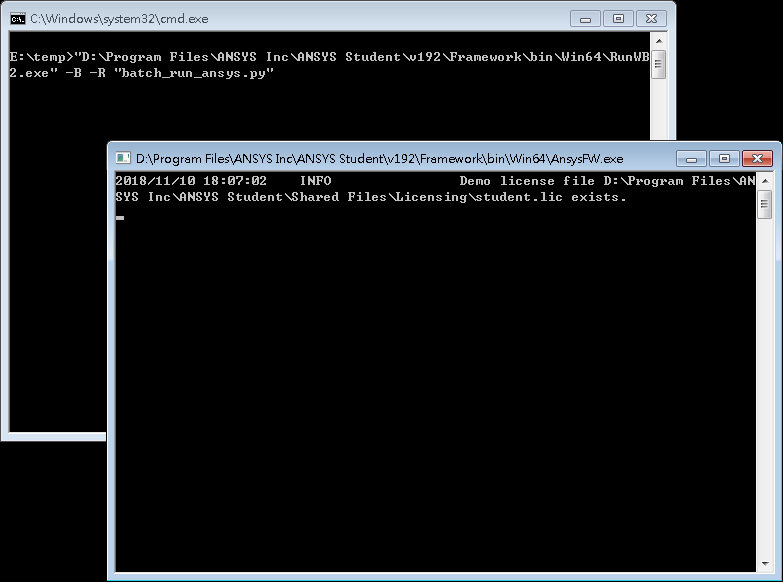
\includegraphics[scale=0.5]{figure/batch.png}
	\caption{Execute batch\_cmd.bat}
	\label{fig:batch}
\end{figure}

\begin{figure}[h]
	\centering
	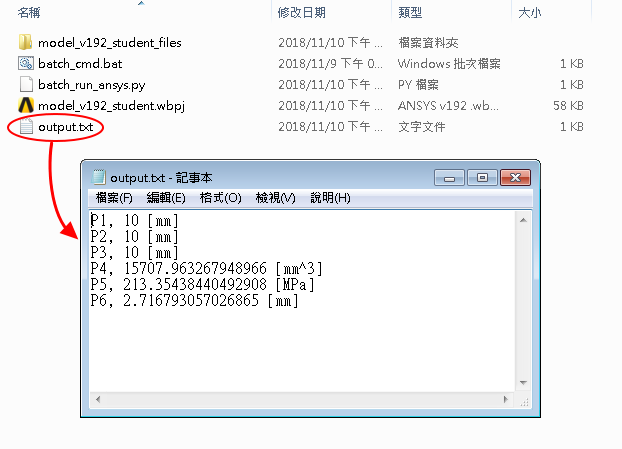
\includegraphics[scale=0.6]{figure/output.png}
	\caption{Output text file}
	\label{fig:output}
\end{figure}

\newpage

% -----------------------------------------------
\clearpage
\end{CJK}
\end{document}
